\documentclass[11pt,a4paper]{article}
\usepackage[T1]{fontenc}
\usepackage{lmodern,microtype}
\usepackage[margin=20mm,headheight=14pt]{geometry}
\usepackage{amsmath,amssymb,mathtools}
\usepackage{booktabs,tabularx,array}
\usepackage{enumitem}
\usepackage{xcolor}
\usepackage{tikz,pgfplots}
\usetikzlibrary{arrows.meta,positioning,calc}
\pgfplotsset{compat=1.18}
\usepackage{fancyhdr}
\usepackage[colorlinks=true,linkcolor=courseblue,urlcolor=courseblue]{hyperref}
\definecolor{courseblue}{HTML}{1F4E8C}
\definecolor{courseteal}{HTML}{247C78}
\definecolor{muted}{HTML}{586575}
\definecolor{softblue}{HTML}{EDF3FA}
\definecolor{softteal}{HTML}{EAF5F1}
\hypersetup{pdftitle={From Text to Attention: Structure and Figure Plan},
  pdfauthor={CS40008.01, Fudan University}}
\pagestyle{fancy}
\fancyhf{}
\lhead{\small CS40008.01 \, / \, Fall 2026}
\rhead{\small First four lectures: notes outline}
\cfoot{\small\thepage}
\renewcommand{\headrulewidth}{0.3pt}
\setlength{\parindent}{0pt}
\setlength{\parskip}{5pt}
\setlist[itemize]{leftmargin=1.3em,itemsep=2pt,topsep=3pt}
\setlist[enumerate]{leftmargin=1.5em,itemsep=2pt,topsep=3pt}
\setcounter{secnumdepth}{0}
\newcolumntype{Y}{>{\raggedright\arraybackslash}X}
\newcommand{\sectionplan}[3]{%
  \section{\texorpdfstring{#1\quad #2}{#1 #2}}
  {\small\color{muted}#3\par}}
\newcommand{\tagline}[1]{\textcolor{courseblue}{\textbf{#1}}}
\newcommand{\figids}[1]{\textcolor{courseteal}{\textbf{Figure plan:} #1}}
\newcommand{\source}[2]{\href{https://github.com/baojian/llm-26-fall/blob/1adbaa5442a567cbd2ab65035b8e485778dd46a9/#1}{#2}}
\newcommand{\R}{\mathbb{R}}
\newcommand{\softmax}{\operatorname{softmax}}
\newcommand{\CE}{\operatorname{CE}}
\newcommand{\BOS}{\textsc{bos}}
\newcommand{\EOS}{\textsc{eos}}
\begin{document}
\thispagestyle{empty}
{\small\color{courseblue}\bfseries COURSE NOTES \quad / \quad STRUCTURE AND FIGURE PLAN}

\vspace{8pt}
{\fontsize{29}{33}\selectfont\bfseries From Text to Attention\par}
\vspace{5pt}
{\large Foundations for reading \emph{Attention Is All You Need}\par}
{\color{muted}Lectures 01--04 \quad $\cdot$ \quad September 30, 2026\par}

\textbf{Purpose.} Build a compact, illustrated reference around the computations
students have already encountered. The proposed finished notes have about
\textbf{20--25 core pages}, with short supporting appendices. This document is
the structure and figure plan; it contains two vector figure prototypes.

\textbf{Scope.} Include single-head scaled dot-product attention, causal masking,
and component verification from Lecture 04. End before the full Transformer
architecture. This is a boundary in the course sequence, not a restriction to
methods published before 2017.

\begin{center}
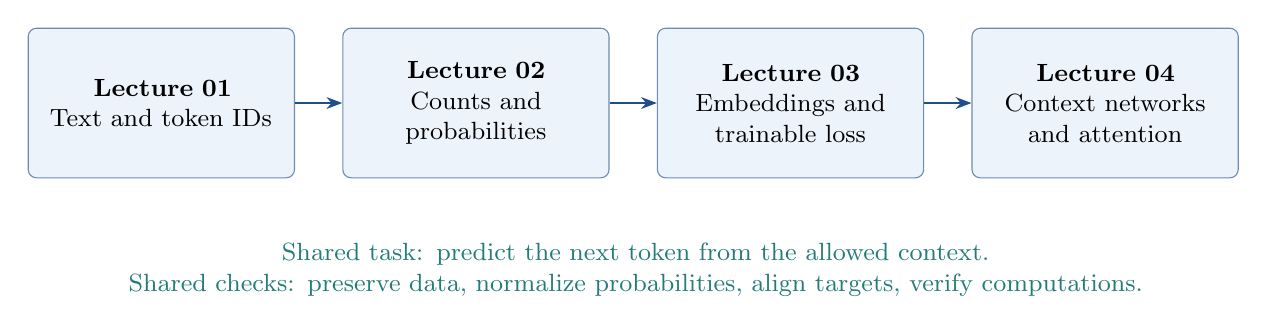
\begin{tikzpicture}[
  node distance=6mm,
  lecture/.style={draw=courseblue!65,fill=softblue,rounded corners=3pt,
    text width=31mm,minimum height=19mm,align=center,font=\small,inner sep=4pt},
  flow/.style={-{Stealth[length=2mm]},line width=.8pt,draw=courseblue}
]
\node[lecture] (l1) {\textbf{Lecture 01}\\Text and token IDs};
\node[lecture,right=of l1] (l2) {\textbf{Lecture 02}\\Counts and probabilities};
\node[lecture,right=of l2] (l3) {\textbf{Lecture 03}\\Embeddings and trainable loss};
\node[lecture,right=of l3] (l4) {\textbf{Lecture 04}\\Context networks and attention};
\draw[flow] (l1)--(l2);
\draw[flow] (l2)--(l3);
\draw[flow] (l3)--(l4);
\node[below=7mm of $(l2.south)!0.5!(l3.south)$,align=center,
  text width=145mm,font=\small,text=courseteal] {
  Shared task: predict the next token from the allowed context.\\
  Shared checks: preserve data, normalize probabilities, align targets, verify computations.
};
\end{tikzpicture}

\end{center}
{\small\color{muted}\textbf{Prototype F01.} The lectures progressively change
the representation and context computation while retaining a normalized
next-token objective and explicit checks.}

\subsection{Proposed contents}
\renewcommand{\arraystretch}{1.16}
\begin{tabularx}{\textwidth}{@{}r Y l r@{}}
\toprule
& Section & Main source & Pages\\
\midrule
1 & Language modeling as a common task & L01--L02 & 1\\
2 & From text to tokens & L01 & 3--4\\
3 & Count-based language models & L02 & 2--3\\
4 & Evaluating and sampling language models & L02 & 2--3\\
5 & Learning token representations & L03 & 3\\
6 & From token IDs to a trainable neural LM & L02--L04 & 4\\
7 & Representing longer context & L04 & 1--2\\
8 & Attention, causality, and verification & L04 & 4--5\\
\bottomrule
\end{tabularx}

\textbf{Writing pattern.} For each major idea, use a question, a diagram,
one equation or algorithm, a small worked example, and a check that can fail.
Group related panels to keep the finished notes near the page target.

\textbf{Figure budget.} Specify 32 figures or panels: conceptual diagrams in
TikZ and numerical plots exported as vector PDF. F01 and F29 are prototyped
here; the remaining entries are authoring plans.

\clearpage
\sectionplan{1}{Language modeling as a common task}{L01 introduction; L02 distribution matching and chain rule \quad / \quad about 1 page}
\tagline{Question: What do all of these language models try to predict?}
\begin{itemize}
  \item Start with a short reminder of language tasks and the difference
  between a fluent response and a checked answer. Compress the historical
  survey to a paragraph.
  \item Define a corpus, token sequence, model distribution, and prediction
  event. State the sampling assumptions behind an empirical objective.
  \item Connect KL minimization, expected log likelihood, empirical
  negative log likelihood, and the exact chain-rule factorization.
\end{itemize}
\[
p_\theta(x_{1:T})=\prod_{t=1}^{T}p_\theta(x_t\mid x_{<t}),
\qquad
\mathcal L(\theta)=-\frac{1}{N_{\rm pred}}
\sum_{\text{scored events}}\log p_\theta(x_t\mid x_{<t}).
\]
Explain that sequence-averaged and token-averaged objectives use different
weighting when document lengths vary. Use token averaging for the metric
ledger in these notes.

\textbf{Check.} Identify what is observed, what is predicted, which parameters
are shared, and whether the stated conditional distribution sums to one.

\figids{F01 course map; F08 chain-rule diagram shared with Section 3.}

\sectionplan{2}{From text to tokens}{L01 preprocessing, Unicode, BPE, and held-out comparisons \quad / \quad 3--4 pages}
\tagline{Question: What information reaches the model, and what can be recovered?}
\begin{enumerate}
  \item \textbf{Corpus and preprocessing.} Sources, coverage, train/dev/test
  separation before fitting; extraction versus lossless partitioning; regular
  expressions and allowed merge boundaries.
  \item \textbf{Representations of text.} Visible symbols, Unicode code
  points, UTF-8 bytes, token occurrences, token types, and token IDs.
  Contrast NFC, NFKC, and lowercasing.
  \item \textbf{Byte-level BPE training.} Weighted adjacent-pair counts,
  deterministic tie handling, non-overlapping replacements, vocabulary
  growth, and boundaries. Work through the existing
  \texttt{low}$\times5$, \texttt{lower}$\times2$ example.
  \item \textbf{Encoding with a frozen tokenizer.} Apply learned merge
  ranks; concatenate token bytes before UTF-8 decoding; distinguish text
  from special/control tokens. Briefly locate other tokenizer families.
  \item \textbf{Vocabulary and sequence tradeoffs.} Coverage and held-out
  token counts by language; connect vocabulary rows and sequence length
  to costs developed later.
\end{enumerate}
\textbf{Checks.} The round trip recovers the original text only when no
irreversible normalization was applied. Pair counts can include overlaps
even though replacements cannot. The lecture's weighted token totals are
$25\to18\to11$ after two merges; compression alone does not establish LM quality.

\figids{F02--F07: pipeline, Unicode, boundaries, BPE, frozen encoding,
and vocabulary/sequence tradeoffs.}

\clearpage
\sectionplan{3}{Count-based language models}{L02 estimation and smoothing \quad / \quad 2--3 pages}
\tagline{Question: How can we estimate a next-token distribution from counts?}
\begin{enumerate}
  \item Contrast the exact chain rule with the finite-history approximation:
  unigram, bigram, trigram, and the general $(n-1)$-token history.
  \item Extract sentence-local events; define \BOS, \EOS, output vocabulary,
  unknown tokens, counts, and maximum-likelihood estimates.
  \item Explain the zero-probability problem, additive smoothing,
  interpolation, and development-set tuning. Give backoff/Kneser--Ney
  one short contextual paragraph, matching its limited lecture treatment.
\end{enumerate}
\[
\widehat p_{\rm MLE}(w\mid h)=\frac{c(h,w)}{c(h)},\qquad
p_\delta(w\mid h)=\frac{c(h,w)+\delta}{c(h)+\delta K}.
\]
Here $K$ is the number of possible output symbols, including \EOS\ when it
is scored; the MLE expression requires $c(h)>0$. Specify behavior for unseen
histories before using a mixture:
\[
p(w\mid h)=\sum_{r=0}^{n}\lambda_r p_r(w\mid h),
\qquad \lambda_r\geq0,\quad \sum_r\lambda_r=1.
\]
Use $p_0$ for a uniform floor and $p_r$ for the order-$r$ component,
with a normalized fallback for unseen histories.
\textbf{Worked example.} Reuse the three-sentence corpus from L02 E01 and
L03's opening recap: after \texttt{I}, counts are \texttt{am}:2 and
\texttt{do}:1, yielding $2/3$ and $1/3$.

\textbf{Checks.} Normalize each conditional distribution, prevent
cross-document pairs, distinguish raw MLE zeros from a smoothed scorer,
and use the same distribution for sampling and scoring.

\figids{F08--F10: histories, counts-to-probabilities, and smoothing.}

\sectionplan{4}{Evaluating and sampling language models}{L02 evaluation, sampling, and pipeline demonstrations \quad / \quad 2--3 pages}
\tagline{Question: What does a better score mean, and what can it fail to show?}
\begin{itemize}
  \item Use development data for choices and a fixed test set for final
  comparisons. Relate intrinsic likelihood to task-specific evaluation.
  \item Derive the metric conversions from total negative log likelihood
  $S=-\sum\ln p_\theta(x_t\mid x_{<t})$ in nats:
  $N$ scored predictions and $B_{\rm utf8}$ evaluated text bytes.
  \[
  \ell=S/N,\quad {\rm PPL}=e^\ell,\quad
  {\rm BPT}=\ell/\ln2,\quad {\rm BPB}=S/(B_{\rm utf8}\ln2).
  \]
  \item Interpret the uniform-distribution baseline, branching factor,
  and why per-token perplexity cannot directly compare tokenizers.
  Keep preprocessing, evaluated text, boundaries, and special-token
  conventions identical for a BPB comparison.
  \item Explain categorical sampling with cumulative intervals, then
  autoregressive generation from \BOS\ to \EOS.
\end{itemize}
\textbf{Application box.} Retain the reference-LM data filter and the
sample/retrain loop as concise demonstrations of experimental reasoning.
The filter score is not a universal quality label. The self-training run
changes token budget, truncation, and sampling; it does not isolate one cause.

\figids{F11--F14: metric units, tokenizer comparison, sampling, and
the two pipeline demonstrations.}

\clearpage
\sectionplan{5}{Learning token representations}{L03's bounded classical bridge and lookup material \quad / \quad about 3 pages}
\tagline{Question: What makes representations useful, and what objective learns them?}
\begin{enumerate}
  \item Move from context-count rows to association:
  $\operatorname{PPMI}(w,c)=\max\{0,\log_2[p(w,c)/(p(w)p(c))]\}$.
  Reuse the \texttt{tea}/\texttt{coffee}/\texttt{car} table.
  \item Show low-rank compression by SVD and briefly contrast GloVe's
  weighted log-count objective. Avoid presenting them as the same method.
  \item Contrast CBOW and skip-gram prediction directions, center/context
  tables, and observed-versus-sampled pair discrimination.
  \item Work one negative-sampling gradient by hand and check it with
  autograd. Explain that this pairwise loss is not normalized LM likelihood.
  \item Introduce fastText's character n-gram composition, with a small
  comparison to BPE segmentation. Distinguish static token vectors,
  context-dependent states, and retrieval vectors.
\end{enumerate}
\[
\ell_{\rm NS}=-\log\sigma(\mathbf w^\top\mathbf c_+)
             -\log\sigma(-\mathbf w^\top\mathbf c_-),\qquad
\nabla_{\mathbf c_+}\ell_{\rm NS}
=(\sigma(\mathbf w^\top\mathbf c_+)-1)\mathbf w .
\]
\textbf{Check.} A close neighbor or an analogy result is an observation
about vector geometry; it does not substitute for held-out LM evaluation.
Keep the bridge proportional to the ten slides actually taught.

\figids{F15--F19: count geometry, prediction direction, gradient,
representation types, and subword composition.}

\sectionplan{6}{From token IDs to a trainable neural LM}{L02 NPLM introduction; L03 mechanics; L04 fixed-window model \quad / \quad about 4 pages}
\tagline{Question: Can we trace every tensor and every update?}
\begin{itemize}
  \item Define lookup as selecting rows of $E\in\R^{K_{\rm in}\times d}$,
  and show its one-hot matrix-product equivalent. State shape, dtype, and
  device; distinguish input rows from the $K$ possible output symbols.
  \item Trace the L03 neural bigram: selected vector, vocabulary readout,
  raw logits, softmax, shifted targets, and cross-entropy.
  \item Extend the same computation to L04's ordered $m$-token context:
  \[
  u=\operatorname{concat}(E[x_{t-m}],\ldots,E[x_{t-1}]),\quad
  h=\tanh(W_hu+b_h),\quad z=W_oh+b_o .
  \]
  \item Explain stable log-sum-exp, label-preserving reshapes, autograd,
  gradient clearing, backpropagation, and the optimizer step.
  Use a detached-loss example and a compatible tiny-batch fit.
  \item Contrast training fit with a held-out coverage probe; distinguish
  evaluation mode from disabling gradient recording.
  \item Explain weight tying with compatible row meanings and widths,
  both gradient paths, unique parameter
  counts, optimizer-state payload, logits storage, and projection work.
\end{itemize}
\textbf{Checks.} Zero logits give $\ln K$ loss. L03's model still conditions
on one token. L04's fixed-window network can distinguish prefixes sharing
the last token. An fp32 Adam parameter/gradient/two-moment subtotal uses
16 bytes per parameter, excluding activations and other overhead.

\figids{F20--F25: tensor path, stable loss, context capacity, fit/probe,
weight tying, and resource ledger.}

\clearpage
\sectionplan{7}{Representing longer context}{L04's short recurrence and attention-motivation bridge \quad / \quad 1--2 pages}
\tagline{Question: Which information can reach a prediction?}
\begin{enumerate}
  \item Compare an explicit fixed window with a recurrent state updated
  through the prefix. Use one unrolled diagram with shared weights:
  $h_t=\tanh(W_xe_t+W_hh_{t-1}+b)$.
  \item Explain products of local Jacobians. Label $0.9^{50}$ and
  $1.1^{50}$ as scalar illustrations, not measured recurrent gradients.
  \item Give the purpose of LSTM gates using
  $c_t=f_t\odot c_{t-1}+i_t\odot\widetilde c_t$.
  Keep the full gate and BPTT derivations in supporting reading.
  \item Explain the fixed-vector bottleneck of early encoder--decoder
  translation models and the idea of consulting stored source states.
\end{enumerate}
\textbf{Historical distinction.} Bahdanau et al.'s additive attention
motivates query-dependent context selection. It is not the scaled dot-product
self-attention mechanism implemented next.

\figids{F26--F27: alternative context paths and query-dependent selection.}

\sectionplan{8}{Attention, causality, and verification}{L04 single-head computation and tests \quad / \quad 4--5 pages}
\tagline{Question: Can a query select context without reading the future?}
\begin{enumerate}
  \item Start from a weighted sum of values, then introduce learned
  queries, keys, and values with explicit dimensions.
  \[
  Q=XW_Q,\quad K_{\!a}=XW_K,\quad V_{\!a}=XW_V,\qquad
  A=\softmax_{\rm row}\!\left(\frac{QK_{\!a}^{\top}}{\sqrt{d_k}}+M\right),
  \quad Y=AV_{\!a}.
  \]
  \item Compute the three-position example from L04: scores, stable
  row-wise softmax, and value contributions. Explain the scaling rationale
  and avoid treating weights as a complete causal explanation.
  \item Align position $t$ with target $x_{t+1}$; permit keys $j\leq t$.
  Set disallowed scores to $-\infty$ before normalization.
  \item Compare a vectorized head with a transparent reference:
  outputs, parameter/input gradients, finite differences, normalized rows,
  and future-input perturbation tests.
  \item Account for one materialized score tensor:
  $b_{\rm elem}BT^2$ bytes per head. For $B=1$ and fp32, lengths
  $512,1024,2048$ require $1,4,16$ MiB for that tensor.
  \item End with order information and the familiar
  embedding--context--readout--loss path. A paired key/value permutation
  leaves a fixed query's sum unchanged when the allowed set is unchanged;
  this does not make an entire causal network permutation invariant.
\end{enumerate}
\textbf{Stopping point.} Students can explain and verify one causal head.
The next reading introduces multi-head composition, positional representations,
residual paths, normalization, feedforward sublayers, and the full 2017
encoder--decoder architecture.

\figids{F28--F32: Q/K/V, numerical attention, mask, verification, and cost.}

\clearpage
\section{Figure inventory: text, counts, and representations}
{\small Each entry identifies the explanatory job and the existing source.
\textit{PDF plot} means an original numerical plot generated from course data,
not a screenshot of a slide.}

\begingroup
\small
\renewcommand{\arraystretch}{1.23}
\begin{tabularx}{\textwidth}{@{}p{8mm} Y >{\raggedright\arraybackslash}p{32mm}@{}}
\toprule
ID & Figure or paired panels and the question they answer & Form / source\\
\midrule
F01 & Four-lecture map: what changes between representations, context computation, and prediction? & TikZ / course structure\\
F02 & Raw bytes, decoding, normalization, chunking, IDs, and reconstruction. At which step can information be lost? & TikZ / L01 pipeline\\
F03 & Visible symbol, code points, UTF-8 bytes, tokens: why can the counts differ? Include the accented-letter example. & TikZ / L01 E03\\
F04 & Regex extraction versus a lossless partition, with allowed BPE boundaries. Which characters survive? & TikZ / L01 P01\\
F05 & Weighted BPE pair table and two merge steps; an overlap inset. Why is pair count not always the token reduction? & TikZ / L01 E04\\
F06 & Frozen merge ranks applied to an unseen word. Why does encoding differ from retraining? & TikZ / L01 E05\\
F07 & Vocabulary/sequence cost sketch beside held-out language token counts. What changes with tokenizer training data? & TikZ + PDF / L01 E06\\
F08 & Chain-rule factors above unigram, bigram, and trigram context windows. Which part is an approximation? & TikZ / L02 model\\
F09 & Sentence-local pairs, count matrix, normalized row, and a next-token draw. How do counts become probabilities? & TikZ / L02 E01, L03 recap\\
F10 & Raw counts, add-$\delta$, and an interpolated distribution. Where does probability mass for unseen events come from? & PDF plot / L02 P02--P03\\
F11 & One total negative log likelihood converted into nats/token, bits/token, perplexity, and bits/byte. What is the denominator? & TikZ / L02 metrics note\\
F12 & The same four bits over four versus two tokens, with a shared byte count. Why can perplexity comparisons mislead? & TikZ / L02 metrics note\\
F13 & Cumulative sampling intervals, then the append-and-repeat loop. Does the sampler use the scored distribution? & TikZ / L02 P01\\
F14 & Reference-score filtering and sample/retrain diagrams, with the actual token budgets shown. What would a controlled comparison hold fixed? & TikZ + PDF / L02 experiment JSON\\
F15 & Context counts, PPMI heatmap, and rank-two table. What signal is retained or compressed? & PDF plot / L03 toy counts\\
F16 & CBOW versus skip-gram arrows and two parameter tables. What predicts what? & TikZ / L03 classical bridge\\
\bottomrule
\end{tabularx}
\endgroup

\textbf{Use existing evidence.} L01's plots come from
\path{sequence-length.json} and \path{heldout-chinese.json}.
L02's numerical applications come from \path{lecture02-results.json},
\path{lm-filter.json}, and \path{self-training-loop.json}.
L03's count/PPMI fixture is \path{counts-ppmi.json}.
These files live in the corresponding lecture's assets directory.

\clearpage
\section{Figure inventory: training, context, and attention}
\begingroup
\small
\renewcommand{\arraystretch}{1.23}
\begin{tabularx}{\textwidth}{@{}p{8mm} Y >{\raggedright\arraybackslash}p{32mm}@{}}
\toprule
ID & Figure or paired panels and the question they answer & Form / source\\
\midrule
F17 & One positive and one sampled pair, score, loss, and a gradient arrow. Which parameter moves, and why? & TikZ / L03 E02\\
F18 & Token ID, selected embedding row, contextual state, and retrieval vector. Which representation changes with context? & TikZ / L03 E01 and bridge\\
F19 & Character n-gram composition beside BPE segmentation. How are fastText subwords different from tokenizer output? & TikZ / L03 fastText slide\\
F20 & IDs to lookup to context to vocabulary logits to shifted-target loss, with all tensor shapes. Where can alignment fail? & TikZ / L03 E01, E03\\
F21 & Computation graph for stable log-sum-exp and cross-entropy, plus a disconnected-loss branch. Which operations preserve gradients? & TikZ / L03 stability, L04 E02\\
F22 & Neural bigram versus a two-token NPLM on prefixes sharing the last token. Which model can separate the examples? & TikZ / L03 limitation, L04 E01\\
F23 & Tiny-batch training curves beside a separate coverage probe. What has the fit established? & PDF plot / L03 E04, L04 E02\\
F24 & Untied and tied tables with both gradient paths. Why do shared rows receive multiple contributions? & TikZ / L03 E05\\
F25 & Parameter, gradient, Adam-moment, and logit-storage ledger; a projection-work panel. What does each subtotal omit? & PDF plot / L03 E06\\
F26 & Fixed window, unrolled recurrence, and a gated memory path. How does earlier information reach the output? & TikZ / L04 recurrence\\
F27 & Fixed encoder vector versus query-weighted stored source states. Which bottleneck does attention address? & TikZ / L04 historical bridge\\
F28 & Q/K/V projections, score matrix, row normalization, value aggregation, and shapes. Which axis indexes keys? & TikZ / L04 Q/K/V\\
F29 & Scores $(1,0,1)$, masked/unmasked weights, and resulting vectors. What does removing future access change? & TikZ/PGFPlots / L04 E03--E04\\
F30 & Lower-triangular allowed cells aligned with shifted targets; contrast masking before and after softmax. Which rows are normalized? & TikZ / L04 E04\\
F31 & Forward comparison, gradient comparison, finite differences, and future-input perturbation. Which bug can each catch? & TikZ / L04 E05\\
F32 & Linear token-state storage versus quadratic materialized score storage, with the $1,4,16$ MiB examples. Which tensor is counted? & PDF plot / L04 P01\\
\bottomrule
\end{tabularx}
\endgroup

\textbf{Numerical provenance.} Use the two distinct
\texttt{tiny-lm-loss.json} files for the L03 and L04 experiments; label
their different models, vocabulary sizes, and training batches.
F29--F31 use L04's \texttt{attention-values.json} and verified notebook cells.
Use consistent source data rather than tracing plotted pixels.

\clearpage
\section{Prototype F29: one query, with and without a causal mask}
The query is $q_2=(\sqrt2,0)$ with $d_k=2$. The hand-chosen vectors in the
Lecture 04 fixture are:
\[
K_{\!a}=\begin{bmatrix}1&0\\0&1\\1&1\end{bmatrix},
\qquad
V_{\!a}=\begin{bmatrix}1&0\\0&2\\3&1\end{bmatrix}.
\]
Hence $q_2K_{\!a}^{\top}/\sqrt{d_k}=(1,0,1)$.
Position 2 may access positions 1 and 2 in causal next-token prediction.

\begin{center}
% Values recomputed from slides/lecture-04/assets/attention-values.json.
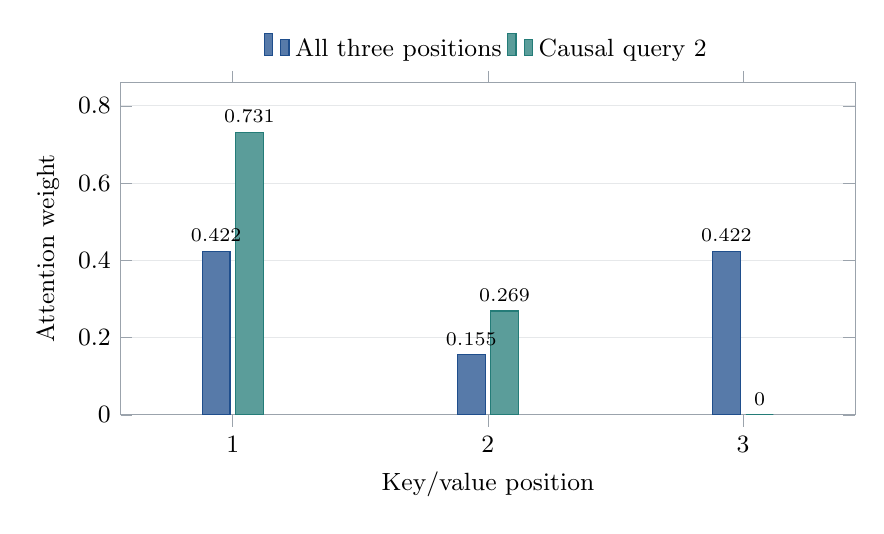
\begin{tikzpicture}
\begin{axis}[
  width=.9\textwidth,height=58mm,
  ybar,bar width=10pt,
  ymin=0,ymax=.86,
  symbolic x coords={1,2,3},xtick=data,
  xlabel={Key/value position},ylabel={Attention weight},
  ytick={0,.2,.4,.6,.8},
  tick label style={font=\small},label style={font=\small},
  legend style={font=\small,at={(.5,1.03)},anchor=south,legend columns=2,
    draw=none,fill=none},
  axis line style={draw=muted!60},tick style={draw=muted!60},
  ymajorgrids,grid style={draw=muted!15},
  nodes near coords,
  every node near coord/.append style={font=\scriptsize,
    /pgf/number format/fixed,/pgf/number format/precision=3},
  enlarge x limits=.22,
]
\addplot[fill=courseblue!75,draw=courseblue]
  coordinates {(1,.4223187983) (2,.1553624035) (3,.4223187983)};
\addplot[fill=courseteal!75,draw=courseteal]
  coordinates {(1,.7310585786) (2,.2689414214) (3,0)};
\legend{All three positions,Causal query 2}
\end{axis}
\end{tikzpicture}

\end{center}

\begin{align*}
a_2^{\rm full}&\approx(0.422319,\;0.155362,\;0.422319),&
y_2^{\rm full}&\approx(1.689275,\;0.733044),\\
a_2^{\rm causal}&\approx(0.731059,\;0.268941,\;0),&
y_2^{\rm causal}&\approx(0.731059,\;0.537883).
\end{align*}
\textbf{A falsifiable check.} Changing $v_3$ by $(10,10)$ changes the
unmasked output by approximately $(4.223188,4.223188)$ and leaves the
causal output unchanged. This example changes a value vector while holding
the query and keys fixed. The full implementation also tests future
\emph{input} perturbations and gradients.

{\small\color{muted}\textbf{Source.}
\source{slides/lecture-04/assets/attention-values.json}{Lecture 04's original toy fixture};
the vectors are hand-chosen, not learned representations or a benchmark.
The diagram is editable TikZ/PGFPlots and compiles to vector graphics.}

\subsection{Figure production conventions}
\begin{itemize}
  \item Use TikZ for computation graphs, token strips, masks, and dependency
  diagrams. Use generated vector PDFs for numerical curves and heatmaps.
  \item Give each figure one explanatory question and a caption stating its
  assumptions, dimensions or units, source, and the conclusion it supports.
  \item Keep blue for representations/probabilities, teal for permitted
  context or verified paths, and gray for masked or inactive elements.
  Include labels or line styles so color is not the only cue.
  \item Set final-size labels at 9--11 points. Keep notation identical to
  the text. Label counts, probabilities, nats, bits, bytes, and MiB explicitly.
  \item Record seeds, step indexing, split, and model size for empirical
  curves. Keep toy examples and measured experiments visibly identified.
\end{itemize}

\clearpage
\section{Notation and reusable source structure}
\begin{tabularx}{\textwidth}{@{}l Y@{}}
\toprule
Symbol & Convention for the finished notes\\
\midrule
$x_t$ & Token ID at position $t$; prediction from position $t$ targets $x_{t+1}$\\
$K_{\rm in},K$ & Input-table rows and possible output symbols; declare special-token conventions for each example\\
$B,T$ & Batch size and sequence length; $B_{\rm utf8}$ counts evaluated bytes\\
$d,m,H$ & Embedding width, fixed context length, and hidden width\\
$E,W_o$ & Input table and vocabulary readout; state orientations beside shapes\\
$Q,K_{\!a},V_{\!a}$ & Attention queries, keys, and values; subscripts avoid confusing keys with vocabulary size\\
$d_k,d_v,A,M$ & Key/value widths, attention weights, and additive score mask\\
\bottomrule
\end{tabularx}

\subsection{Suggested layout when expanding this outline}
\begin{verbatim}
docs/first-four-lectures/
  main.tex                 # finished notes
  sections/
    01-language-modeling.tex
    02-text-and-tokenization.tex
    03-count-language-models.tex
    04-evaluation-and-sampling.tex
    05-representation-learning.tex
    06-neural-language-models.tex
    07-longer-context.tex
    08-attention-and-causality.tex
  figures/                 # editable TikZ sources
  plots/                   # deterministic vector-PDF generators
  references.bib
  outline.tex              # this reviewable plan
\end{verbatim}
Build products belong under the repository's ignored \texttt{output/pdf/}
directory. The present draft includes \texttt{outline.tex}, two figure sources,
a Makefile, and a README; the remaining files above are the proposed layout.

\subsection{Writing order and supporting appendices}
\begin{enumerate}
  \item Fix notation, evaluation conventions, and the running examples.
  Draft Sections 1--4 and their representation/counting diagrams.
  \item Draft Sections 5--6 around the checked token-to-loss computation,
  keeping the classical bridge short.
  \item Draft Sections 7--8, add component checks, and finish with the
  explicit boundary before the Transformer paper.
\end{enumerate}
Supporting appendices can contain a regex/Unicode reference, extra
count and smoothing arithmetic, longer classical-embedding and recurrent
derivations, and a PyTorch debugging/shape checklist. Use the same notes and
expectations for all students.

\clearpage
\section{Coverage and source map}
The source of coverage is the published Fall course at commit
\texttt{1adbaa5}. The lecture decks and checked classroom notebooks take
priority over broader Spring materials and optional readings.

\begin{tabularx}{\textwidth}{@{}l Y@{}}
\toprule
Lecture & Source and use in this outline\\
\midrule
L01 & \source{slides/lecture-01/teaching-plan.md}{Teaching plan},
\source{slides/lecture-01/slides.md}{slides},
\source{slides/lecture-01/lecture-01-exercise.ipynb}{classroom notebook}.
Sections 1--2; retain preprocessing/BPE examples and held-out token counts.\\
L02 & \source{slides/lecture-02/teaching-plan.md}{Teaching plan},
\source{slides/lecture-02/slides.md}{slides},
\source{slides/lecture-02/lecture-02-exercise.ipynb}{notebook}.
Sections 1, 3--4, and the NPLM motivation in Section 6.\\
L03 & \source{slides/lecture-03/teaching-plan.md}{Teaching plan},
\source{slides/lecture-03/slides.md}{slides},
\source{slides/lecture-03/lecture-03-exercise.ipynb}{notebook}.
Sections 5--6; preserve the bounded classical bridge and neural-bigram limitation.\\
L04 & \source{slides/lecture-04/teaching-plan.md}{Teaching plan},
\source{slides/lecture-04/slides.md}{slides},
\source{slides/lecture-04/lecture-04-exercise.ipynb}{notebook}.
Sections 6--8; preserve fixed-window training, attention, and verification.\\
\bottomrule
\end{tabularx}

\subsection{Existing supplementary course notes}
\begin{itemize}
  \item \source{docs/lecture-01-pre-tokenization.md}{Lecture 01 preprocessing reader}:
  use selected explanations; keep the larger corpus-engineering inventory
  as supporting reading.
  \item \source{docs/lecture-02-lm-metrics.md}{Lecture 02 metrics note}:
  use the unit conversions and evaluation conventions.
  \item \source{slides/lecture-03/classical-reading.md}{Lecture 03 classical reading}
  and \source{slides/lecture-04/optional-reading.md}{Lecture 04 optional reading}:
  sources for appendices, not evidence that all derivations were covered in class.
\end{itemize}

\subsection{Primary reading anchors}
\begin{itemize}
  \item Sennrich, Haddow, and Birch (2016).
  \href{https://aclanthology.org/P16-1162/}{Neural Machine Translation of Rare Words with Subword Units}.
  BPE as a subword method; distinguish the paper's setup from the course's byte-level example.
  \item Bengio et al.\ (2003).
  \href{https://www.jmlr.org/papers/v3/bengio03a.html}{A Neural Probabilistic Language Model}.
  Jointly learned representations and a fixed-window conditional model.
  \item Mikolov et al.\ (2013).
  \href{https://arxiv.org/abs/1301.3781}{Efficient Estimation of Word Representations in Vector Space};
  \href{https://papers.nips.cc/paper_files/paper/2013/file/9aa42b31882ec039965f3c4923ce901b-Paper.pdf}{Distributed Representations of Words and Phrases and their Compositionality}.
  Prediction directions and negative sampling.
  \item Bahdanau, Cho, and Bengio (2015; preprint 2014).
  \href{https://arxiv.org/abs/1409.0473}{Neural Machine Translation by Jointly Learning to Align and Translate}.
  Motivation for consulting stored source states.
  \item Vaswani et al.\ (2017).
  \href{https://arxiv.org/abs/1706.03762}{Attention Is All You Need}.
  The next paper; its single-head attention computation has already been introduced in L04.
\end{itemize}
\end{document}
